\titledquestion{Maximum area rectangle in histogram}

We are given a histogram consisting of $n$ parallel bars side by side, each of width $1$, as well as a sequence $A$ containing the heights of the bars where the height of the $i$th bar is $\mathbf{a}_i$ for $\forall \; i \in [n]$. For example, the figures below show the case where $n= 7$ and $A = \langle 6, 2, 5, 4, 4, 1, 3 \rangle$. Our goal is to find the maximum area of the rectangle placed inside the boundary of the given histogram with a \textbf{divide-and-conquer} algorithm. (Here you don't need to find which rectangle maximizes its area.)

Reminder: There do exist algorithms that solve this problem in linear time. However, you are \textbf{not allowed} to use them in this homework. Any other type of algorithms except the divide-and-conquer ones will get \textbf{no} credit.

\begin{figure}[htbp]
    \centering
    \begin{minipage}[t]{0.48\textwidth}
        \centering
        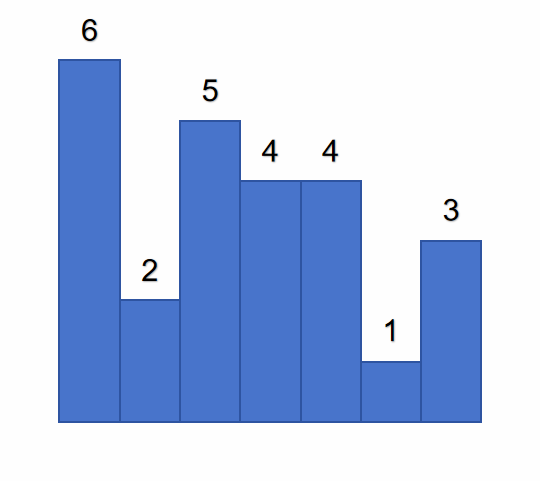
\includegraphics[width=6cm]{withnum.png}
        \caption{The Original Histogram}
    \end{minipage}
    \begin{minipage}[t]{0.48\textwidth}
        \centering
        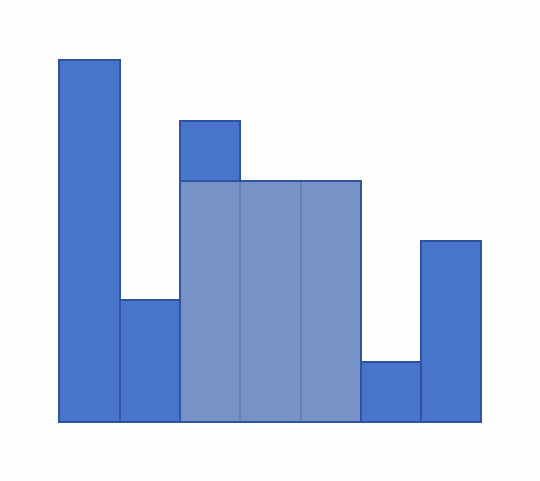
\includegraphics[width=6cm]{withrect.png}
        \caption{The Largest Rectangle in Histogram}
    \end{minipage}
\end{figure}

You may use $Rect(l, r, A)$ to represent the answer of the sub-problem w.r.t. the range $\left[l, r\right]$.

\begin{parts}
    \part[3] \textbf{Briefly} describe:
    \begin{enumerate}
        \item How would you divide the original problem into 2 sub-problems?
        \item Under what circumstances will the answer to the original problem not be covered by the answers of the 2 sub-problems?
        \item Given the answers of the 2 sub-problems, how would you get the answer of the original problem?
    \end{enumerate}

    \begin{solution} \\
        %%%%%%%%%%%%%%%%%%%%%%%%%%%%%%%%%%%%%%%%%%%%%%%%%
        % Replace `\vspace{2in}' with your answer.
        %\vspace{2in}
        For problem one and three,
        \begin{enumerate}
            \item Choose the first minimum and divide the array into two parts.
                  Part one cotains the elements on the left of first minimum, and the other elements without the first element form the other part.
            \item Update the answer, which is 0 at the begining, with the larger one between the length of subarray multiply minimum and the answer.
            \item Repeat the operations above for every subarray.
        \end{enumerate}
        For problem two, \\
        If the array is strictly ascending or descending, the problem will not be divided into two subproblems.
        %%%%%%%%%%%%%%%%%%%%%%%%%%%%%%%%%%%%%%%%%%%%%%%%%
    \end{solution}

    \newpage

    \part[8] Based on your idea in part(a), design a \textbf{divide-and-conquer} algorithm for this problem. Make sure to provide \textbf{clear description} of your algorithm design in \textbf{natural language}, with \textbf{pseudocode} if necessary.

    \begin{solution}
        %%%%%%%%%%%%%%%%%%%%%%%%%%%%%%%%%%%%%%%%%%%%%%%%%
        % Replace `\vspace{7.5in}' with your answer.
        %\vspace{7.5in}
        \begin{enumerate}
            \item Find the minimum called $m_1$, with position $pos$.
            \item Update the answer with $m_1 * n$.
            \item Divide the array A into two parts. One is A from head to $pos-1$, called $A_1$ and the other is A from $pos+1$ to tail, called $A_2$.
            \item Find the minimum in $A_1$ called $m_2$ and its position.
            \item Update the answer with $max(answer, m_2 * (pos-head))$.\
            \item Divide the array $A_1$ into two parts in the same way as A.
            \item Repeat the operations above through recrusion, and end progressing if the length of $A_i$ is $1$.
        \end{enumerate}
        \textbf{Pseudocode:}\\
        $A$ is the original array with length n. $head$ and $tail$ is the head address or tail address of array A.
        \begin{algorithm}[H]
            \color{blue}
            \begin{algorithmic}[1]
                \State answer = 0
                \Function{$find\_min$}{A, head, tail}
                \State min = A[0]
                \State pos = head
                \State \For{i=1,$i<n$,i++}
                \State \State \If{$min > A[i]$}
                \State \State \State min = A[i]
                \State \State \State pos = i
                \State \State \EndIf
                \State \EndFor
                \State \Return pos
                \EndFunction
                \Function{$maximum\_area$}{A, head, tail}
                \State pos = $find\_min$(A, head, tail)
                \State answer = max(A[pos]*(tail-head+1), answer)
                \If {head == tail}
                \State \Return answer
                \EndIf
                \If {pos == head}
                \State \Return max(answer, $maximum\_area$(A, pos+1, tail))
                \ElsIf {pos == tail}
                \State \Return max(answer, $maximum\_area$(A, head, pos-1))
                \Else
                \State \Return max($maximum\_area$(A, head, pos-1), $maximum\_area$(A, pos+1, tail))
                \EndIf
                \EndFunction
            \end{algorithmic}
        \end{algorithm}
        %%%%%%%%%%%%%%%%%%%%%%%%%%%%%%%%%%%%%%%%%%%%%%%%%
    \end{solution}

    \newpage

    \part[2] Provide the run-time complexity analysis of your algorithm in part (b). Make sure to include the \textbf{recurrence relation} of the run-time in your solution.

    \begin{solution}
        %%%%%%%%%%%%%%%%%%%%%%%%%%%%%%%%%%%%%%%%%%%%%%%%%
        % Replace `\vspace{3in}' with your answer.
        %\vspace{3in}
        For the minimum in array, the expected position is $\sum_{i=0}^{n-1} \frac{i}{n}$, which is the middle.
        Thus the problem will be divided into two equal parts in expectation. In the function $maximum_area$ without
        recrusion, the time complexity is $\theta(n)$ since we should find the minimum. Thus, we have
        \begin{equation}
            T(n) = 2T(\frac{n}{2}) + \theta(n)
        \end{equation}
        According to the master therom, the whole time complexity is $\theta(nlogn)$.
        %%%%%%%%%%%%%%%%%%%%%%%%%%%%%%%%%%%%%%%%%%%%%%%%%
    \end{solution}

\end{parts}